\chapter{Modelo de datos}
\label{ch:modelo_datos}

\begin{figure}[H]
    \centering
    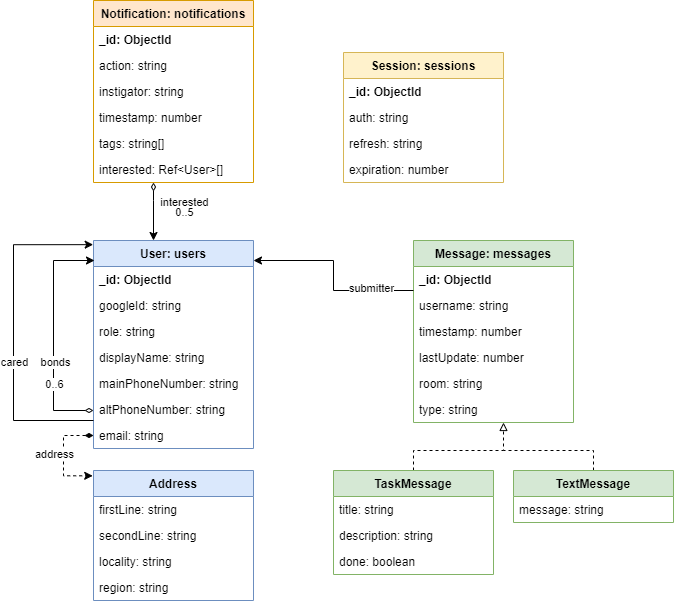
\includegraphics[width=1\textwidth]{images/Diseño/ModeloDatos.drawio.png}
    \caption{Diagrama del modelo de datos}
    \label{fig:diagrama_modelo_datos}
\end{figure}

\section{Mensaje}

Dentro de los mensaje se aúnan dos entidades de la aplicación: los \textbf{mensajes de texto} que se envían a través del Feed y las \textbf{tareas}, que también pueden ser enviadas a través del mismo. Todos estos mensajes se almacenan en la colección \emph{messages}. Aunque se puede poner en duda la elección de tratar las tareas como mensajes, esta decisión de diseño parte de un aprovechamiento de la flexibilidad de las bases de datos documentales como la que se emplea en el sistema.

Las consultas para obtener las entidades del Feed en caso de utilizar colecciones diferentes para los mensajes de texto y las tareas habría implicado la necesidad de realizar \emph{\glspl{join}}, que aunque es una operación soportada por MongoDB en sus últimas versiones, es un claro indicativo de un modelo de datos mal diseñado para bases de datos no relacionales como la nuestra. Es por eso que tanto tareas como mensajes son \textbf{incluidas en la misma colección} y tratadas ambas como mensajes al nivel de lógica de la \acrshort{api}.

\subsection{BaseMessage}

De cara a favorecer una compatibilidad lo mayor posible entre los dos tipos de entidades que se guardarán en la colección se define una primera entidad con campos comunes a ambas y que serán necesarios en las consultas a la colección. Tanto los mensajes de texto como las tareas contarán con todas las propiedades de esta clase base. Véase \fref{sch:message}.

\begin{itemize}
    \item \textbf{id}: \emph{string}. Obligatorio. Identificador único del mensaje. Generada automáticamente por MongoDB al persistir la entidad por primera vez.
    \item \textbf{submitter}: \emph{User}. Obligatorio. Referencia al usuario creador del mensaje.
    \item \textbf{username}: \emph{string}. Obligatorio. Nombre público del autor en el momento de la creación. Cacheado en este documento para evitar la necesidad de hacer \emph{\glspl{join}} con la colección de usuarios para acceder a este dato y optimizar las consultas con este tipo de base de datos.
    \item \textbf{timestamp}: \emph{number}. Obligatorio. Instante de creación del mensaje.
    \item \textbf{lastUpdate}: \emph{number}. Obligatorio. Instante de la última actualización del mensaje, si no se ha actualizado nunca desde su creación su valor será el mismo que el de \textbf{timestamp}.
    \item \textbf{room}: \emph{string}. Obligatorio. Identificador de la sala de mensajería a través de la que fue enviado el mensaje.
    \item \textbf{type}: \emph{string}. Obligatorio. Tipo de mensaje, puede ser: Text o Task.
\end{itemize}

\subsection{TaskMessage}
\label{ssec:task_message}

Representa las tareas creadas por los usuarios, tanto en la vista de Tareas como a través del Feed. Hereda de BaseMessage y su tipo es \textbf{Task}. Véase \fref{sch:task_message}. Además de las propiedades de BaseMessage cuenta con las siguientes:

\begin{itemize}
    \item \textbf{title}: \emph{string}. Obligatorio. Título de la tarea.
    \item \textbf{description}: \emph{string}. Opcional. Descripción de la tarea.
    \item \textbf{done}: \emph{boolean}. Obligatorio. Estado de la tarea, a \code{true} es hecha y \code{false} es no hecha.
\end{itemize}

\subsection{TextMessage}
\label{ssec:text_message}

Representa los mensajes de texto simples enviados a través del Feed. Hereda de BaseMessage y su tipo es \textbf{Text}. Véase \fref{sch:text_message}. Además de las propiedades de BaseMessage tiene la siguiente propiedad:

\begin{itemize}
    \item \textbf{message}: \emph{string}. Obligatorio. Cuerpo del mensaje.
\end{itemize}

\section{Notificación}

Las notificaciones reflejan una \textbf{acción de interés} para una serie de usuarios. Dicha acción se almacena en la entidad y es una de una enumeración conocida. Como algunas de estas acciones pueden servirse más de una vez, para aportar más contexto cuentan un campo para añadir etiquetas que podrán ser almacenadas y leídas según fuese necesario con cada tipo de acción.

Por otro lado, las notificaciones son \textbf{entidades compartidas} por una serie de usuarios. Los usuarios a notificar son almacenados en la entidad para su recuperación por parte de estos, una vez que un usuario marque como leída la notificación su ID será eliminada de esa lista de usuarios, de forma que la entidad pase a ir dirigida únicamente a aquellos usuarios que aún no la leyesen. Cuando una notificación ha sido leída por todos sus usuarios asociados será eliminada de la base de datos.

Las notificaciones se almacenan en la colección \emph{notifications}. El esquema definitivo se puede ver en el \fref{sch:notification}. Sus propiedades son:

\begin{itemize}
    \item \textbf{id}: \emph{string}. Obligatorio. Identificador único de la notificación. Generada automáticamente por MongoDB al persistir la entidad por primera vez.
    \item \textbf{action}: \emph{Action}. Obligatorio. Acción notificada, puede ser una de las listadas en \fref{class:api:action}.
    \item \textbf{instigator}: \emph{string}. Obligatorio. Nombre del usuario que provocó la acción a notificar.
    \item \textbf{timestamp}: \emph{number}. Obligatorio. Instante en el que ocurrió la acción.
    \item \textbf{tags}: \emph{string array}. Lista de cadenas de texto con información adicional de la notificación. Por defecto existirá como lista vacía.
    \item \textbf{interested}: \emph{User array}. Lista de referencias a los usuarios que son notificados y que aún no han leído la notificación.
\end{itemize}

\section{Sesión}
\label{ssec:sesion}

De cara a gestionar las sesiones y validar e invalidar los \glspl{token} de forma correcta, se ha creado también una colección para el almacenamiento de estas llamada \emph{sessions} (véase \fref{sch:session}). Las propiedades almacenadas son:

\begin{itemize}
    \item \textbf{id}: \emph{string}. Obligatorio. Identificador único de la sesión. Generada automáticamente por MongoDB al persistir la entidad por primera vez.
    \item \textbf{auth}: \emph{string}. Obligatorio. Es el \gls{token} activo de la sesión.
    \item \textbf{refresh}: \emph{string}. Obligatorio y único. Es el \gls{token} que permite refrescar la sesión de usuario sin necesidad de volver a autenticarse.
    \item \textbf{expiration}: \emph{number}. Obligatorio. Instante de expiración de la sesión, equivalente al tiempo de validez del \gls{token} de autenticación. Almacenado para limpiar sesiones caducadas de la base de datos.
\end{itemize}

\section{Usuario}

Los usuarios son las entidades clave de la aplicación. Su esquema en la base de datos (véase \fref{sch:user}) contiene toda la información de cada usuario, así como sus relaciones con otros usuarios. No existe una entidad diferente para Pacientes y Cuidadores. Las diferencias se gestionarán en el servicio, por lo que la entidad contiene tanto la lista de vínculos de los Pacientes como el campo para almacenar el vínculo de un Cuidador. Tiene las siguientes propiedades:

\begin{itemize}
    \item \textbf{id}: \emph{string}. Obligatorio. Identificador único del usuario. Generada automáticamente por MongoDB al persistir la entidad por primera vez.
    \item \textbf{googleId}: \emph{string}. Obligatorio y único. \Gls{token} de usuario de la cuenta de Google del usuario. Almacenada para autenticar al usuario con su cuenta de Google, no es recuperada de la base de datos al no tener ningún otro uso.
    \item \textbf{role}: \emph{Role}. Obligatorio. Rol del usuario, puede ser cualquiera de los listados en \fref{class:api:role}.
    \item \textbf{displayName}: \emph{number}. Opcional. Nombre visible del usuario.
    \item \textbf{mainPhoneNumber}: \emph{string}. Opcional. Número de teléfono principal del usuario.
    \item \textbf{altPhoneNumber}: \emph{string}. Opcional. Número de teléfono alternativo del usuario.
    \item \textbf{address}: \emph{Address}. Opcional. Dirección postal del usuario (véase \fref{ss:address}).
    \item \textbf{email}: \emph{string}. Opcional. Dirección electrónica del usuario.
    \item \textbf{bonds}: \emph{User array}. Opcional. Lista de referencias a los usuarios vinculados con un Paciente.
    \item \textbf{cared}: \emph{User}. Opcional. Referencia al Paciente vinculado de un Cuidador.
\end{itemize}

\subsection{Address}
\label{ss:address}

Representación de las direcciones postales como objetos del sistema, compuesta por las siguientes propiedades:

\begin{itemize}
    \item \textbf{firstLine}: \emph{string}. Opcional. Primera línea de la dirección para la información principal.
    \item \textbf{secondLine}: \emph{string}. Opcional. Segunda línea de la dirección para la información principal.
    \item \textbf{locality}: \emph{string}. Opcional. Localidad.
    \item \textbf{region}: \emph{string}. Opcional. Región.
\end{itemize}